\documentclass[11pt,letterpaper]{article}
\usepackage[utf8]{inputenc}
\usepackage{float, xcolor}

%----- Configuración del estilo del documento------%
\usepackage{graphicx, fancyhdr, lastpage}
\usepackage[left=2cm,right=2cm,top=1.8cm,bottom=2.3cm]{geometry}

\pagestyle{fancy}
\fancyhf{}
\rfoot{\textit{Página \thepage \hspace{1pt} de \pageref{LastPage}}}

%------ Paquetes matemáticos básicos --------%
\usepackage{amsmath, amssymb, amsthm}

\begin{document}

%------ Encabezado -------- %
\begin{center}
  \begin{minipage}{3cm}
    \begin{center}
      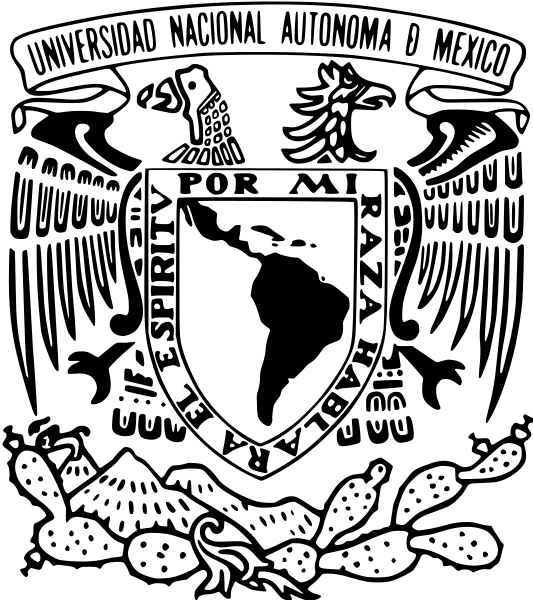
\includegraphics[height=3.4cm]{unam_logo.png}
    \end{center}
  \end{minipage}\hfill
  \begin{minipage}{10cm}
    \begin{center}
      \textbf{\Large Universidad Nacional Autónoma de México}\\[0.2cm]
      \textbf{\large Facultad de Ciencias}\\[0.2cm]
      \textbf{Lógica Computacional | 2025-2}\\[0.4cm]
      \textbf{\Large Tarea 01}\\[0.1cm]
      \textbf{Docentes:}\\
      Noé Hernández \hspace{1em} Santiago Escamilla \hspace{1em} Ricardo López\\[0.3cm]
      \textbf{Autores:}\\
      Fernanda Ramírez Juárez \quad Ianluck Rojo Peña\\[0.3cm]
      \textbf{Fecha de entrega:} Miércoles 12 de febrero de 2025
    \end{center}
  \end{minipage}\hfill
  \begin{minipage}{3cm}
    \begin{center}
      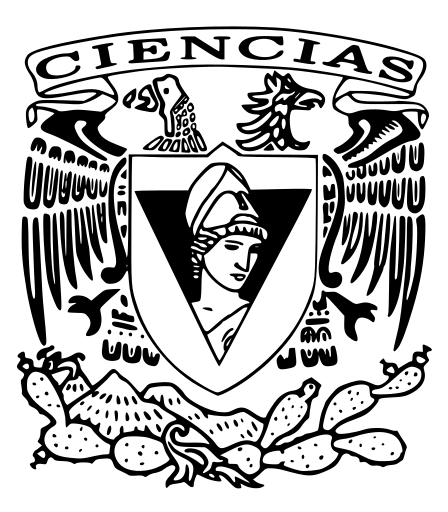
\includegraphics[height=3.4cm]{fc_logo.png}
    \end{center}
  \end{minipage}
\end{center}

\bigskip
\hrule height 0.1pt
\bigskip

%------ Notas sobre la resolución --------%
\section*{Notas sobre la resolución}

\begin{quote}
  \textbf{Nota general:}  
  Los ejercicios fueron resueltos en base a las notas de clase (IcNota2.pdf) y a los comentarios dados en las sesiones del curso. Se tomaron en cuenta los siguientes puntos específicos:  
\end{quote}

\begin{itemize}
   \item \textbf{Ejercicios 1 y 2:} Se basan en las notas del profesor y los comentarios del 30 de enero y 6 de febrero.  
   \item \textbf{Ejercicio 4:} Resuelto con base en la sección '7. Conceptos semánticos básicos' en IcNota2.pdf y explicaciones del ayudante Santiago el 7 de febrero.
   \item \textbf{Ejercicio 5:} Derivado de un ejercicio resuelto en clase el 30 de enero.
   \item \textbf{Ejercicio 6:} Link a la página de apoyo para realizar el ejercicio: https://sites.google.com/ciencias.unam.mx/estructuras-discretas-2024-2/clases/notas-de-clase?authuser=0
   \item \textbf{Ejercicio 6 y 7:} Se basan en las clases y notas del profesor además las clases del ayudante Santiago los días 6, 7, 10, 11 y 12 de febrero.
\end{itemize}

\bigskip
\hrule height 0.1pt
\bigskip

%------ Contenido -------- %
\section*{Resolución de Ejercicios}

\begin{enumerate}
  
  % ---- Ejercicio 1 ----
  \item (1.5 pt.) Usando las siguientes claves:
    \begin{itemize}
       \item $p :=$ María está contenta.
       \item $q :=$ María pide una bicicleta por su cumpleaños.
       \item $r :=$ María recibe una bicicleta por su cumpleaños.
       \item $s :=$ María odia a Juan.
       \item $t :=$ Juan va a la playa.
       \item $u :=$ Juan está de vacaciones.
       \item $v :=$ El sol brilla.
    \end{itemize}
    
    Exprese en español las siguientes fórmulas llenando el cuadro que está abajo.
    
    \begin{enumerate}
       \item Siempre que María está contenta y el sol brilla, deja de odiar a Juan.
       \item Cuando brilla el sol, Juan va a la playa, si está de vacaciones.
       \item María está contenta siempre que Juan está de vacaciones y se va a la playa.
       \item Aunque María está contenta porque pidió una bicicleta para su cumpleaños y la ha recibido, odia a Juan.
       \item María recibirá una bicicleta en su cumpleaños sólo si la pide.
    \end{enumerate}
    
    \bigskip

    \begin{table}[H]
      \begin{center}
        \begin{tabular}{| c | c | c | c | c | c |}
          
          \hline 
          & $(u \land t) \rightarrow p$ & $\neg (r \land \neg q )$ & $(p \land v) \rightarrow \neg s$ & $(p \land (q \land r)) \land s$ & $v \rightarrow u \rightarrow t$ \\ \hline
          1 & & & \checkmark & & \\ \hline
          2 & & & & & \checkmark \\ \hline
          3 & \checkmark & & & & \\ \hline
          4 & & & & \checkmark & \\ \hline
          5 & & \checkmark & & & \\ \hline
        \end{tabular}
      \end{center}
    \end{table}

    \bigskip
    
  % ---- Ejercicio 2 ----
  \item (1 pt.) Desarrolle las siguientes sustituciones, además elimine los paréntesis que sean redundantes según el orden de precedencia de los operadores lógicos visto en clase:
    
    \begin{itemize}
    \item[\textbf{a})] $\left( (\neg (p \land q) \leftrightarrow \left( (\neg q) \rightarrow (p \rightarrow s) \right) \right) \quad [p := (q \rightarrow s)] [s := (\neg p)]$ \\
      \\
      Sustituímos a la variable atómica $p$ con la fórmula \( (q \rightarrow s) \) en la proposición:
      \[
      \left(( \neg ((q \rightarrow s) \land q)) \leftrightarrow \left( (\neg q) \rightarrow ((q \rightarrow s) \rightarrow s \right) \right)) \quad [s := (\neg p)]
      \]
      Ahora continuamos con la sustitución de $s$:
      \[
      \left(( \neg ((q \rightarrow s) \land q)) \leftrightarrow \left( (\neg q) \rightarrow ((q \rightarrow ( \neg p)) \rightarrow (\neg p)) \right) \right)
      \]
      Por jerarquía de operadores eliminamos los paréntesis innecesarios:
      \[
      \textcolor{blue}{(} \textcolor{magenta}{(}\neg ((q \rightarrow s) \land q) \textcolor{magenta}{)} \leftrightarrow \textcolor{green}{(} \textcolor{orange}{(}\neg q \textcolor{orange}{)} \rightarrow \textcolor{cyan}{(}(q \rightarrow \textcolor{orange}{(} \neg p \textcolor{orange}{)} ) \rightarrow \textcolor{orange}{(} \neg p \textcolor{orange}{)} \textcolor{cyan}{)} \textcolor{green}{)} \textcolor{blue}{)}
      \]
      \[
      = \neg ((q \rightarrow s) \land q) \leftrightarrow \neg q \rightarrow (q \rightarrow \neg p) \rightarrow \neg p
      \]
      
      \textbf{Resultado final:}
      \[
      \neg ((q \rightarrow s) \land q) \leftrightarrow \neg q \rightarrow (q \rightarrow \neg p) \rightarrow \neg p
      \]
      
      \bigskip
      
    \item[\textbf{b})] $\left( (p \lor q) \rightarrow ((\neg r) \leftrightarrow p) \right) \quad [r, p, q := p, q, r]$ \\
      \\
      Dado que es una única sustitución, se reemplazan las variables una vez:
      \[
      \left((q \lor r) \rightarrow \left(( \neg p) \leftrightarrow q\right) \right)
      \]
      Eliminamos los paréntesis:
      \[
      \textcolor{blue}{(} \textcolor{magenta}{(} q \lor r \textcolor{magenta}{)} \rightarrow ( \textcolor{orange}{(} \neg p \textcolor{orange}{)} \leftrightarrow q) \textcolor{blue}{)}
      \]

      \textbf{Resultado final:}
      \[
      q \lor r \rightarrow (\neg p \leftrightarrow q)
      \]
    \end{itemize}
    
    \bigskip

  % ---- Ejercicio 3 ----
  \item (1 pt.) Tomando en cuenta la sintaxis para las fórmulas de la lógica proposicional definida en la Nota 01, reinserte tantos paréntesis como sea posible a la fórmula: $(q \rightarrow p \rightarrow \neg r \land s) \lor \neg p$ \\
    \\
    \[
    (q \rightarrow p \rightarrow \neg r \land s) \lor \neg p = \textcolor{blue}{(}(q \rightarrow \textcolor{magenta}{(} p \rightarrow \textcolor{green}{(} \textcolor{orange}{(} \neg r \textcolor{orange}{)} \land s \textcolor{green}{)} \textcolor{magenta}{)}) \lor \textcolor{orange}{(}\neg p \textcolor{orange}{)} \textcolor{blue}{)}
    \]
    
    \textbf{Resultado final:}
    \[
    ((q \rightarrow (p \rightarrow ((\neg r) \land s))) \lor (\neg p))
    \]
    
  \bigskip

  % ---- Ejercicio 4 ----
  \item (2 pts.) Sean $\Gamma$ y $\Delta$ dos conjuntos de oraciones de la lógica proposicional, y sean $\varphi$ y $\psi$ fórmulas de la lógica proposicional. Determine para cada una de las siguientes afirmaciones si es verdadera, con una demostración, o si es falsa, con un contraejemplo.

    \begin{itemize}
    \item Si $\Gamma \vdash \varphi \land \Delta \vdash \varphi$, entonces $\Gamma \cup \Delta \models \varphi$.
      \subsection*{Demostración}

      \textbf{P.D.} $\Gamma \cup \Delta \vDash \varphi$ significa que para toda interpretación $I$ que satisface a $\Gamma \cup \Delta$, $I(\Gamma \cup \Delta) = 1$, entonces también satisface a $\varphi$, $I(\varphi) = 1$. De este modo, consideramos los siguientes casos:

      \subsubsection*{Caso 1: $\Gamma \cup \Delta$ es insatisfacible}

      Usaremos una de las propiedades de la Proposición 7.5 del archivo PDF \textit{IC-Nota02.pdf} para demostrar este caso. Debemos probar lo siguiente:\\

      Sea $\Gamma'$ un conjunto de fórmulas y $\varphi'$ una fórmula. 

      \textbf{P.D.} Si $\Gamma'$ es insatisfacible, entonces $\Gamma'$ $\vDash \varphi'$.

      Recordemos que la relación de consecuencia lógica se entiende a través de una implicación del siguiente modo:
      \[
      \text{Para toda interpretación } I, I(\Gamma') = 1 \rightarrow I(\varphi') = 1.
      \]

      (Fragmento obtenido de las Notas 02)

      Supongamos ahora que $\Gamma'$ es insatisfacible, entonces $I(\Gamma)'$ = 0 para toda interpretación $I$.

      En particular, si suponemos que se cumple $I(\Gamma') = 0 \rightarrow I(\varphi') = 1$.
      
      Tenemos que, en la lógica proposicional, si el antecedente es falso, la implicación es verdadera sin importar la veracidad de la conclusión.
      
      Así, si $\Gamma'$ es insatisfacible, entonces $\Gamma' \vDash \varphi$.\\

      Y $\therefore$ Si $\Gamma \vdash \varphi \land \Delta$ es insatisfacible, entonces $\Gamma \cup \Delta \models \varphi$

      \subsubsection*{Caso 2: $\Gamma \cup \Delta$ es satisfacible}

      \textbf{Subcaso 2.1:} $\varphi \in \Gamma$ o $\varphi \in \Delta$

      Es trivial, ya que como $\varphi$ pertenece a alguno de los dos conjuntos, éste sigue perteneciendo a la unión, es decir, $\varphi \in \Gamma \cup \Delta$.
      
      Dado que $\Gamma \cup \Delta$ es satisfacible, significa que $I(\Gamma \cup \Delta) = 1$.
      
      Por lo tanto, $\forall  \psi \in \Gamma \cup \Delta, I(\psi) = 1$, lo que implica que $\varphi$ es satisfacible.  

      Así, concluimos que $\Gamma \cup \Delta \vDash \varphi$.

      \textbf{Subcaso 2.2:} $\varphi \notin \Gamma$ y $\varphi \notin \Delta$

      Es trivial, ya que nuestro supuesto es que $\Gamma \vDash \varphi$ y $\Delta \vDash \varphi$.
      
      Y cómo $\Gamma \cup \Delta$ es satisfacible, la interpretación $I$ que hace satisfacible a $\Gamma \cup \Delta$ también hace satisfacible a $\varphi$.  

      Por lo tanto, se concluye que: $\Gamma \cup \Delta \vDash \varphi$.

      \bigskip

      \textbf{Conclusión:} Si $\Gamma \vDash \varphi$ y $\Delta \vDash \varphi$, entonces $\Gamma \cup \Delta \vDash \varphi$.

      \bigskip
      
    \item Si $\Gamma \vDash \varphi$ y $\Delta \nvDash \varphi$, entonces $\Gamma \cup \Delta \vDash \varphi$.
      \subsection*{Demostración}

      Por nuestro supuesto, para toda interpretación I tal que $I(\Gamma) = 1$, se tiene que $I(\varphi) = 1$.
      
      Además, existe I' tal que I'($\Delta$) = 1, pero I'($\varphi$) = 0.

      Notemos que $\Gamma \cup \Delta$ es el conjunto con los elementos tanto de $\Gamma$ como de $\Delta$, por lo que cualquier interpretación $I^{*}$ debe satisfacer las fórmulas de $\Gamma$ como de $\Delta$).

      Pero por nuestro supuesto, existe $\psi \in \Gamma$ tal que $I^{*}(\psi) = 1$, y esta interpretación de la fórmula $\psi$ es necesaria para que $\varphi$ sea consecuencia lógica de $\Gamma$.

      Sin embargo, existe al menos $\psi' \in \Delta$ tal que cualquier interpretación $I^{*}(\psi') = 0$ pues $\psi'$ es la fórmula que, al aplicarle alguna interpretación en $\Delta$, hace que $\varphi$ no sea consecuencia lógica de $\Delta$.

      De este modo, no hay interpretaciones que hagan a \( \Gamma \cup \Delta \) satisfacible, pues de lo contrario, se contradicen a nuestro supuesto.

      Por lo tanto, $\Gamma \cup \Delta$ es insatisfacible, y por una propiedad usada en el ejercicio anterior: Si $\Gamma \cup \Delta$ es insatisfacible, entonces $\Gamma \cup \Delta \vDash \varphi$.

      \[
       \therefore \quad Si \quad \Gamma \vDash \varphi \quad y \quad \Delta \nvDash \varphi,\quad entonces \quad \Gamma \cup \Delta \vDash \varphi
      \]
      
    \item Si $\Gamma \nvDash \psi$, entonces $\Gamma \vDash \neg \varphi$.
      
      \subsection*{Contraejemplo}
      
      Por el Lema 7.2 de las notas (ICNota 02.pdf), $\varnothing$ es un conjunto vacío de fórmulas válidas.
      
      Por lo que definimos a  $\psi = p \rightarrow q$ y $\Gamma = \varnothing$.
      
      Por definición, $p \rightarrow q$ no es tautología, entonces $\Gamma \nvDash \psi$, es decir: $\varnothing \nvDash p \rightarrow q$.
      
      Pues recordemos que toda interpretación satisface a $\varnothing$, pero no toda interpretación satisface $p \rightarrow q$.
      
      Así, $\Gamma \nvDash \neg \psi$, es decir: $\varnothing \nvDash \neg (p \rightarrow q)$ y ya que $\neg (p \rightarrow q)$ sigue sin ser tautología.

      Por lo tanto, la afirmación es falsa.
      \bigskip
      
    \end{itemize}

    \bigskip

    \newpage
  % ---- Ejercicio 5 ----
  \item (1.5 pts.) Mediante interpretaciones decida si los siguientes conjuntos de proposiciones son satisfacibles:
    \begin{itemize}
       \item[a)] $\{ p \rightarrow q, (s \lor p) \land \neg q, \neg s \}$\\
      
         Definimos el conjunto de fórmulas:
         \[
         \Gamma = \{ p \rightarrow q, (s \vee p) \land \neg q, \neg s \}
         \]
         donde:
         \[
         \varphi_1 = p \rightarrow q, \quad \varphi_2 = (s \vee p) \land \neg q, \quad \varphi_3 = \neg s
         \]
         Tenemos que $\Gamma$ es satisfacible si existe una interpretación $I$ tal que $I(\varphi) = 1$ para todo $\varphi \in \Gamma$.\\

         Así, evaluamos $I(\varphi_1) = 1$, es decir, $I(p \rightarrow q) = 1$, lo que implica que $I(p) = 0$ o $I(q) = 1$.\\
         
         Si $I(p) = 0$, entonces $I(q)$ puede tomar cualquier valor. Supongamos que $I(q) = 0$.\\

         Ahora, evaluamos $I(\varphi_2) = 1$, es decir, $I((s \vee p) \land \neg q) = 1$.\\
         
         Para que esto se cumpla, se debe cumplir que $I(s \vee p) = 1$ y $I(\neg q) = 1$.\\
         
         Dado que $I(\neg q) = 1$, se tiene que $I(q) = 0$ como habíamos supuesto.\\

         Por otro lado, $I(s \vee p) = 1$ implica que $I(s) = 1$ o $I(p) = 1$.\\
         
         Como habíamos supuesto que $I(p) = 0$, entonces necesariamente $I(s) = 1$.\\

         Sin embargo, evaluando $I(\varphi_3) = 1$, es decir, $I(\neg s) = 1$,
         se deduce que $I(s) = 0$, lo cual contradice la evaluación anterior de $I(s) = 1$.\\

         Dado que llegamos a una contradicción, se concluye que no existe una interpretación que satisfaga todas las fórmulas de $\Gamma$.  

         \[
         \therefore \Gamma \text{ es insatisfacible.}
         \]

         \bigskip
         
       \item[b)] $\{ p \rightarrow q, q \leftrightarrow s, \neg p, \neg s \}$\\
         
         Definimos el conjunto de fórmulas:
         \[
         \Gamma = \{ p \rightarrow q, q \leftrightarrow s, \neg p, \neg s \}
         \]

         donde:

         \[
         \varphi_1 = p \rightarrow q, \quad \varphi_2 = q \leftrightarrow s, \quad \varphi_3 = \neg p, \quad \varphi_4 = \neg s
         \]

         Analizamos la satisfacibilidad del conjunto, evaluando si cada fórmula es satisfacible.\\
         
         Si $I(\varphi_1) = 1$, es decir, $I(p \rightarrow q) = 1$, entonces debe cumplirse que $I(p) = 0$ o $I(q) = 1$.\\
         
         Dado que $I(\varphi_3) = 1$, es decir, $I(\neg p) = 1$, se tiene que $I(p) = 0$.\\
         
         Por lo tanto, $I(p \rightarrow q) = 1$ se cumple para cualquier valor de $I(q)$.\\

         Ahora evaluamos $I(\varphi_2) = 1$, es decir, $I(q \leftrightarrow s) = 1$, lo que implica que $I(q) = I(s)$.\\
         
         Si $I(q) = 0$, entonces $I(s) = 0$.\\

         Por otro lado, $I(\varphi_4) = 1$, es decir, $I(\neg s) = 1$, lo que implica que $I(s) = 0$.\\
         
         Esto es consistente con la evaluación anterior de $I(s) = 0$.\\

         Sin embargo, si asumimos que $I(q) = 1$, entonces $I(s) = 1$ por la equivalencia $q \leftrightarrow s$.\\
         
         Esto contradice la evaluación de $I(\neg s) = 1$, lo que significa que nuestra suposición de $I(q) = 1$ es incorrecta.\\

         Así, tenemos que $I(p) = I(q) = I(s) = 0$, lo cual es consistente con todas las fórmulas.\\

         De este modo, hemos encontrado una interpretación que satisface todas las fórmulas en $\Gamma$

         \[
         \therefore \Gamma \text{ es satisfacible.}
         \]

    \end{itemize}

  \bigskip

  \newpage
  
  % ---- Ejercicio 6 ----
  \item (2 pts.) Usando deducción natural pruebe la validez de los siguientes:

    \begin{itemize}
       \item $p \rightarrow q, q \rightarrow r \lor s, \neg s, p \vdash r$
       \item $\neg p \lor q \vdash p \rightarrow q$
    \end{itemize}

    \begin{center}
      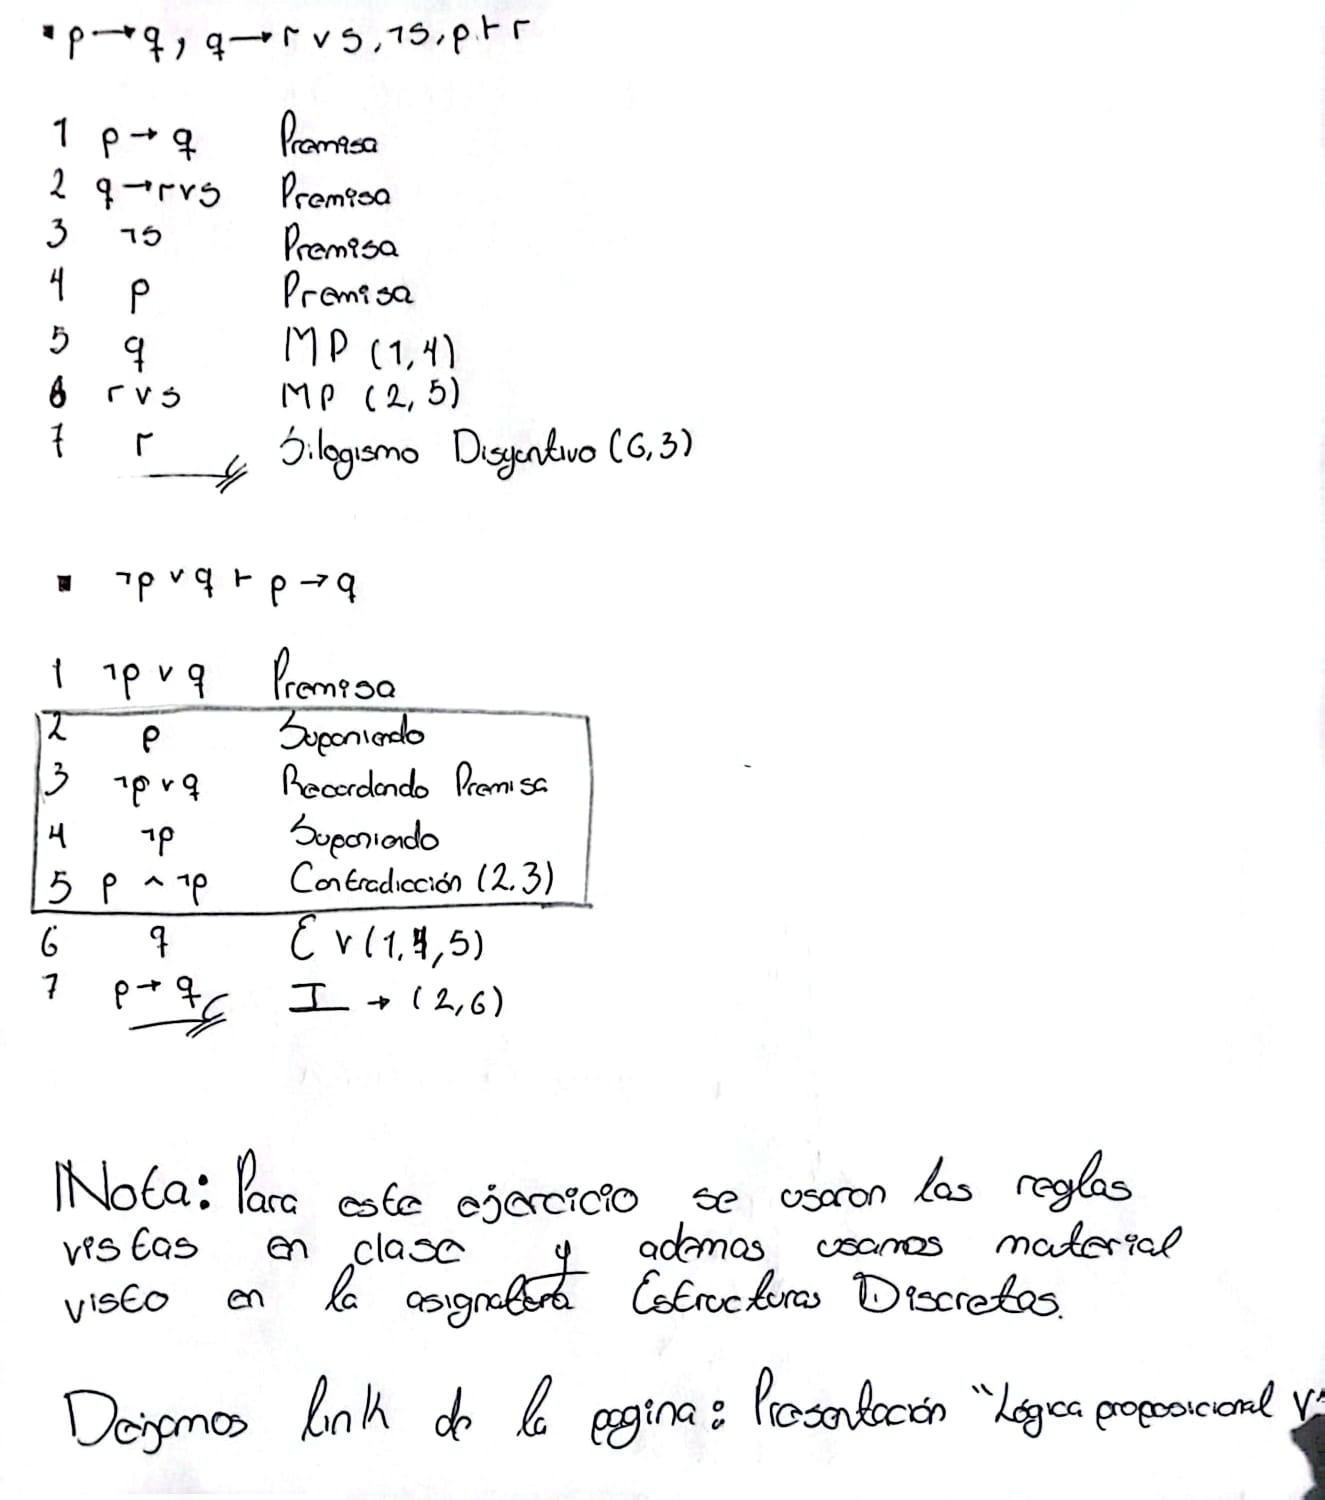
\includegraphics[width=\textwidth,height=0.8\textheight,keepaspectratio]{ejercicio6.png}
    \end{center}
    
  \newpage

  % ---- Ejercicio 7 ----
  \item (2 pts.) Considere el siguiente argumento lógico:

    \textit{Si Sarah Connor destruye a Skynet en 1994, entonces no habrá Día del Juicio Final. Si no hay Día del Juicio Final, John Connor no enviará a su padre a 1984. Es condición necesaria que John Connor envíe a su padre a 1984, para que el mismo John nazca. Sarah Connor no destruye a Skynet en 1994, si John no nace. Por lo tanto, Sarah Connor no destruirá a Skynet en 1994.}

    Tradúzcalo a lógica proposicional y a través de tableaux semánticos determine si es correcto o no.

    \begin{center}
    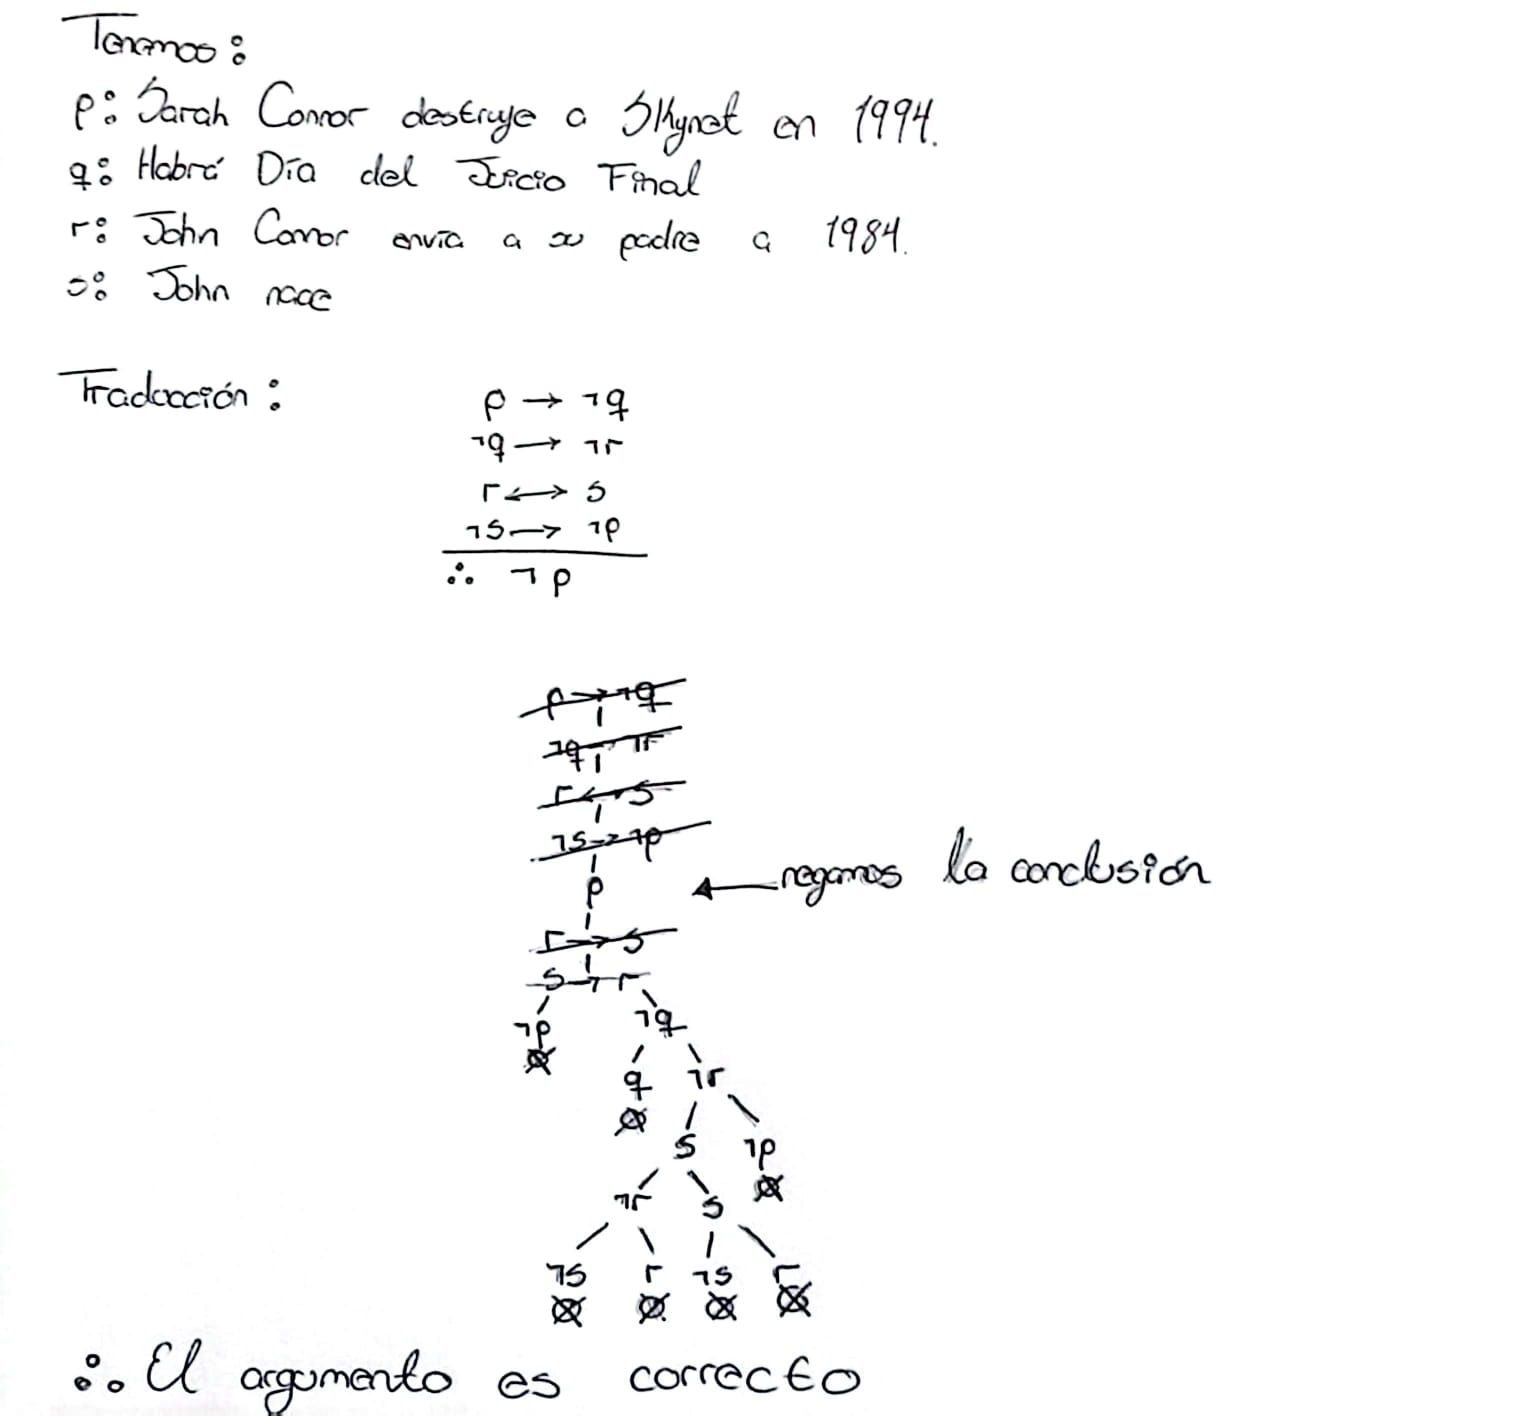
\includegraphics[width=\textwidth,height=0.8\textheight,keepaspectratio]{ejercicio7.png}
    \end{center}
    
\end{enumerate}
\end{document}
